\documentclass[aspectratio=169]{beamer}

\usepackage[utf8]{inputenc}
\usepackage{array}
\usepackage{booktabs}
\usepackage{bold-extra}
\usepackage{graphics}
\usepackage{hyperref}
\hypersetup{%
  colorlinks=true,
  linkcolor=blue,
  filecolor=blue,
  urlcolor=cyan,
}
\usepackage{multicol}
\usepackage{setspace}
\usepackage{verbatim}
\usepackage{fancyvrb} % for verbatim centering

\usetheme{Warsaw}
\usecolortheme{beaver}
\definecolor{clOrange}{HTML}{E76600}
\definecolor{clAlmostWhite}{HTML}{FEFFD9}
\definecolor{clGreen}{HTML}{007F00}
\definecolor{clFlag}{HTML}{D33682}
\definecolor{clFlagOpt}{HTML}{CB4B16}
\definecolor{clRedFlag}{HTML}{DC322F}

\title[LTN03 :: GitBanned]{C-string and C-time functions banned by git}
\author{Adam Graliński}
\date[FFFE\_21]{\textbf{C++ {\color{red}F}{\color{blue}F}{\color{green}F}{\color{yellow}E}, March 2021}}

\setbeamertemplate{navigation symbols}{}
\setbeamercolor{title}{fg=black}
\setbeamercolor{author}{fg=clAlmostWhite}
\setbeamercolor{date}{fg=clAlmostWhite}
\setbeamerfont{author}{size=\huge}
\setbeamerfont{date}{size=\Large}

\begin{document}

{\usebackgroundtemplate{%
 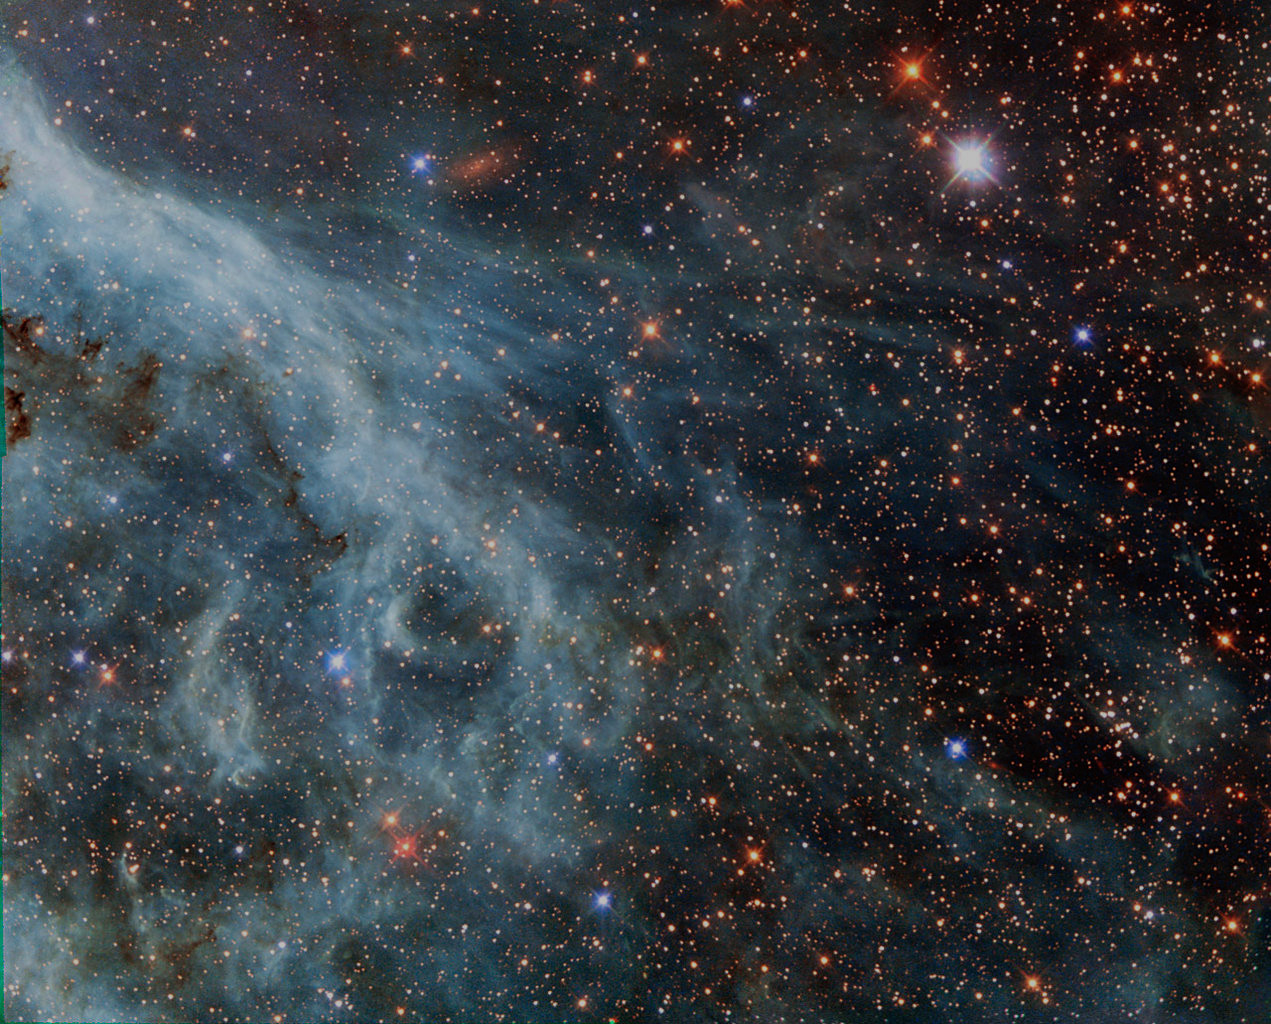
\includegraphics[width=\paperwidth,height=\paperheight]{../common/bg_galaxy.jpg}}
\begin{frame}
\titlepage{}
\end{frame}
}

\begin{frame}
\frametitle{Banned!}
{\Large \href{https://github.com/git/git/blame/master/banned.h}
             {https://github.com/git/git/blame/master/banned.h} bans}
\vspace{1ex}
\begin{itemize}
  \item \texttt{\textbf{strcpy}}
  \item \texttt{\textbf{strcat}}
  \item \texttt{\textbf{sprintf}} and \texttt{\textbf{vsprintf}}
  \item and a bunch of time functions:
  \begin{itemize}
    \item \texttt{\textbf{gmtime}}
    \item \texttt{\textbf{localtime}}
    \item \texttt{\textbf{ctime}} and \texttt{\textbf{ctime\_r}}
    \item \texttt{\textbf{asctime}} and \texttt{\textbf{asctime\_r}}
  \end{itemize}
\end{itemize}
\vspace{1ex}
\begin{flushright}\ldots{}but why?\end{flushright}
\end{frame}


\begin{frame}
\frametitle{strcpy \& strncpy}
{\huge \texttt{\textbf{strcpy}} (and later \texttt{\textbf{strncpy}})}\par
\vspace{4ex}
\begin{itemize}
\item <1->\texttt{strcpy (char* target, const char* source)}
\item <2->\textbf{\textcolor{clRedFlag}{may overflow target}}
\item <3->\texttt{strncpy (char* target, const char* source, size\_t num)}
\item <4->\textbf{\textcolor{clRedFlag}{does not append NUL automatically}}
\item <4->\textbf{clang} warns against using both of these.
\end{itemize}

\vspace{2ex}
{\large Solution: \textcolor{clGreen}{use \texttt{\textbf{snprintf}} instead.}}
\end{frame}


\begin{frame}
\frametitle{strcat \& strncat}
{\huge \texttt{\textbf{strcat}} (and later \texttt{\textbf{strncat}})}\par
\vspace{4ex}
\begin{itemize}
\item <1->\texttt{strcat (char* target, const char* source)}
\item <2->\textbf{\textcolor{clRedFlag}{may overflow target}}
\item <3->\texttt{strncat (char* target, const char* source, size\_t num)}
\item <4->\textbf{\textcolor{clGreen}{fixed: appends NUL automatically, even for truncated entries}}\par

\includegraphics[width=7cm]{pics/strncat_bad.png}
\end{itemize}

\vspace{2ex}
{\large Solution: \textcolor{clGreen}{use \texttt{\textbf{snprintf}} instead.}}
\end{frame}


\begin{frame}
\frametitle{sprintf \& vsprintf}
{\huge \texttt{\textbf{sprintf}} (and later \texttt{\textbf{vsprintf}})}\par
\vspace{4ex}
\begin{itemize}
\item <1->\texttt{sprintf (char* target, const char* format, ...)}
\item <1->\texttt{vsprintf (char* target, const char* format, va\_list arg)}
\item <2->\textbf{\textcolor{clRedFlag}{may overflow target}}
\item <3->\textbf{\textcolor{clGreen}{Scott Meyers, ages ago}}
\end{itemize}

\vspace{2ex}
{\large Solution: \textcolor{clGreen}{use \texttt{\textbf{snprintf}} instead.}}
\end{frame}


\begin{frame}
\frametitle{C-Time}
{\Large What's wrong with:}\par

\begin{table}
\begin{tabular}{l >{\onslide<2->}c<{\onslide} >{\onslide<2->}l<{\onslide}}
  \texttt{\textbf{\textcolor{clRedFlag}{gmtime}}} & &
  \texttt{\textbf{\textcolor{clGreen}{gmtime\_r}}} \\

  \texttt{\textbf{\textcolor{clRedFlag}{localtime}}} & $\rightarrow{}$ &
  \texttt{\textbf{\textcolor{clGreen}{localtime\_r}}} \\

  \texttt{\textbf{\textcolor{clRedFlag}{ctime}}} & &
  \texttt{\textbf{\textcolor{clGreen}{ctime\_r}}} \\

  \texttt{\textbf{\textcolor{clRedFlag}{asctime}}} & &
  \texttt{\textbf{\textcolor{clGreen}{asctime\_r}}} \\
\end{tabular}
\end{table}
\pause{}
Return pointers to static storage (not thread-safe)
\pause{}
\vspace{1ex}
\begin{flushright}\ldots{}when suddenly! $\rightarrow{}$ \end{flushright}
\end{frame}


\begin{frame}
\frametitle{C-Time, again}
\begin{center}
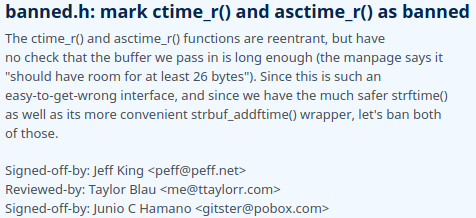
\includegraphics[width=9cm,keepaspectratio]{pics/reentrant_ctime_functions_bad_too.png}
\end{center}
\par{}\vspace{2ex}
{\Large \dots{}just use \textbf{\texttt{strftime}}.}
\end{frame}


\begin{frame}
\frametitle{Summary}
{\huge So\dots}\par
\pause{}
\begin{itemize}[<+->]
  \item C-strings are \textbf{\textcolor{clRedFlag}{hard to use}} and \textbf{\textcolor{clRedFlag}{error-prone}}
  \item C++'s \texttt{\textbf{std::string}}s are a lot easier to use, concatenate, modify*
  \item \texttt{\textbf{snprintf}}: not a silver bullet, but close to
  \item C-time is \textbf{\textcolor{clRedFlag}{easy to do wrong}} too.
\end{itemize}
\vspace{4.5ex}
\begin{center}
\pause{}
{\huge Thank you!}
\end{center}
\end{frame}

\end{document}
